\chapter{The Impact of AGN on Ly\texorpdfstring{$\alpha$}{a} Emission from Massive Halos}
\label{sec:agn}

We now turn our attention to the influence of AGN on our modeled Ly$\alpha$ emission.
Note that from the perspective if the hydrodynamic simulations, black holes are only implemented as sink particles without any feedback (\S~\ref{sec:methods}).
That is, though the black hole particles in this simulation will accrete mass, there is no prescription for the flow of thermal and kinetic energy into the surrounding gas from the accretion, which is what makes black holes astrophysically interesting in this context.
This should be contrasted with our use of an ionizing radiative transfer code to recompute the ionization state in postprocessing due to stars and the UV background.
In both cases this is not self-consistent, but in the previous cases there is already some approximation in the simulations for the energy contribution from these ionizing sources, wheras when we approximate an AGN, we are very self-inconsistent.
But that need not stop us from performing a numerical experiment in postprocessing; it only means that one needs to be cautious in interpreting the results of such an experiment.

Here, we treat AGN as an ionizing source when we compute the ionization state of the gas with {\sc lycrt}.
In this model, the AGN SED is modeled by employing the \citet*{Hopkins2007} templates for unreddened quasars, with the luminosity being tied to the accretion rate via $L = \eta \dot{M_{\rm BH}} c^2$, where $\eta$ is an efficiency parameter with a fiducial value of $\eta = 0.1$.
The impact of the chosen SED model is not particularly important in this work because we do not use it for the ionizing radiative transfer.
The SED informs the rate of ionizing photon emission that is given to {\sc lycrt}, but the emission that is actually used to compute the ionization state follows the aforementioned power law.
For most of this section, we will transform all of the black hole particles in the snapshots into sources for the ionization state calculation.
Sometimes this means there is a very impactful AGN in a satellite galaxy, not the central massive galaxy that the cosmological simulation is oriented around.
In what follows, we investigate the impact of AGN on the total Ly$\alpha$ luminosity, as well as the overall spatial extent of the blob and the blob morphology.

\section{Impact of AGN on Luminosity and Escape Fraction}
In Figure~\ref{fig:agn_recombination_collision} we plot the escaping and intrinsic luminosity due to recombinations and collisions with our approximation for the effects of AGN.
In all cases, we see an increase in emission due to recombinations, and a decrease in emission due to collisional excitation.
Unlike many other observations in this section; this is unsurprising: A gas that experiences a more intense UV field is more ionized and thus favors emission by recombinations (\S~\ref{sec:physicalconcepts}).

As in Figure~\ref{fig:recombination_collision}, the distance between the pale and darker lines provides a visualization of the escape fraction along a median line of sight.
In this case, there is a clear redshift evolution of the escape fraction due to recombinations.
Towards $z=5$, the the escape fraction is very close to $1$, and as the halo evolves it decreases.
This could be explained as a direct consequence of self-shielding and the growth of halo mass over time.
At high redshift, the AGN completely ionizes enough of the surrounding gas 

% TODO Resume here

In Figure~\ref{fig:agn_comparison}, we plot a comparison of the time evolution of the Ly$\alpha$ luminosity, escape fraction, and ionized gas fraction for models with and without an AGN for our fiducial galaxy.
As is evident, there are significant differences in a model that includes AGN compared to one that does not.

When we include a model for AGN (which drives increased ionization in the gas), there are substantial spikes in the luminosity owing to increased emission from recombinations.
This escape fraction enhancement is so substantial than at some orientation angles we can see $f_{\rm esc} > 1$ due to particular geometries that cause Ly$\alpha$ to scatter into the line of sight more than it is absorbed.

Taken together, the increase in the ionization state of the gas (bottom panel of Figure~\ref{fig:agn_comparison}) increases both the emission from recombinations, as well as the escape fraction of Ly$\alpha$ photons.
These combined effects allow for significant boosting ($\sim$ factors of $10-50$) of the Ly$\alpha$ luminosity compared to a no-AGN model.



Since Ly$\alpha$ escape is sightline-dependent we show in Figure~\ref{fig:f_esc} the variation of our fiducial LAB's luminosity and escape fraction over sightlines, with ionization due to AGN and without.
The total luminosity can vary substantially due to the viewing angle of the galaxy when AGN are present.
To demonstrate this explicitly, in the top panel of Figure~\ref{fig:f_esc}, we plot the maximum relative variation between sightlines to show how different a single physical object may appear to an observer who can only view the object from one line of sight.
This huge variation when AGN are present is caused by the distinct non-uniformity of CGM opacity; it's as if the AGN punches large ionization holes in the enclosing CGM through which Ly$\alpha$ readily escapes.
It is important to note that the distribution of escape fractions is not normal, we sample 3072 sightlines to produce this plot which is sufficient to explore all the high-escape pathways out of a LAB.
The top panel of Figure~\ref{fig:f_esc} shows how much variation is possible, and how much the presence of these high-escape sightlines varies over redshift, and the bottom plot shows how dispersed the typical sightlines are.
Because of this sightline variation, an escape fraction (or luminosity) calculated along a single line of sight may not be particularly representative of the overall galaxy properties.

\begin{figure}
    \centering
    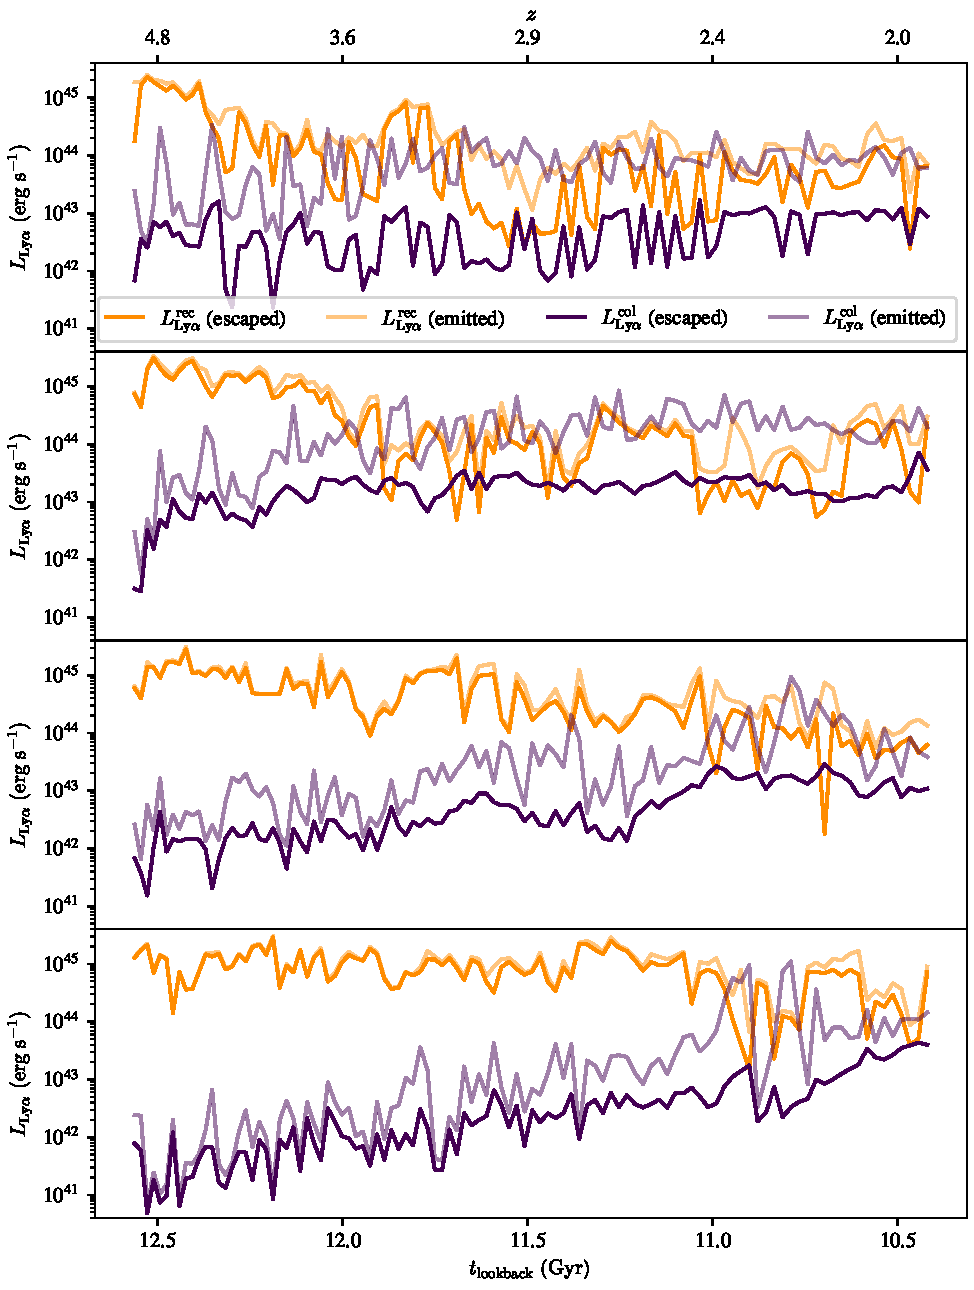
\includegraphics[width=\textwidth,height=\textheight,keepaspectratio]{figures/agn_recombination_collision.pdf}
    \caption{
        All our snapshots broken down by source of emission over redshift; as opposed to Figure~\ref{fig:recombination_collision} this plot includes the effect of AGN.
    }
    \label{fig:agn_recombination_collision}
\end{figure}

\begin{figure}
    \centering
    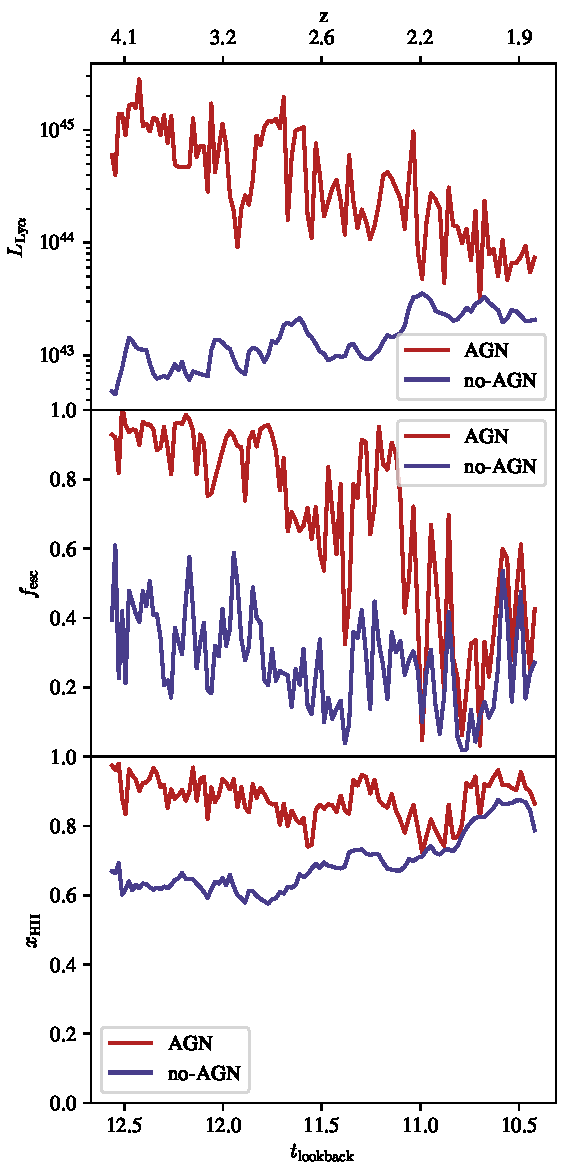
\includegraphics[width=\textwidth,height=\textheight,keepaspectratio]{figures/agn_comparison.pdf}
    \caption{
        We compare the luminosity, escape fraction, and ionization state of the galaxy and halo with and without an AGN model.
        The luminosity of a Ly$\alpha$ blob is sometimes substantially enhanced by the AGN model.
        The simulation domain is always heavily ionized, but the presence of AGN also provides stochastic enhancements, though it does not well correlate with luminosity or escape.
    }
    \label{fig:agn_comparison}
\end{figure}

\begin{figure}
    \centering
    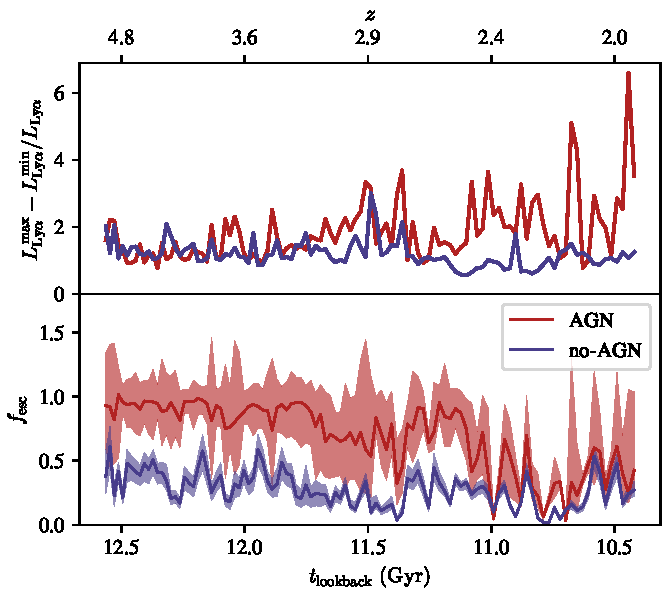
\includegraphics[width=\textwidth,height=\textheight,keepaspectratio]{figures/agn_stats_by_los.pdf}
    \caption{
        Maximum fractional difference between lines of sight (top) and escape fraction (bottom) over redshift for a MassiveFIRE galaxy that forms a LAB, with and without AGN.
        The solid lines on the bottom plot show the median escape fraction over all lines of sight and the shaded region around them show the 1-$\sigma$ variation in that quantity over various lines of sight.
}
    \label{fig:f_esc}
\end{figure}

\begin{figure}
    \centering
    \includegraphics[width=\textwidth,height=\textheight,keepaspectratio]{figures/many_los.pdf}
    \caption{
        A single snapshot, seen from 12 equally spaced lines of sight.
    }
    \label{fig:many_los}
\end{figure}


\section{The impact of AGN on the spatial extent and concentration of Ly\texorpdfstring{$\alpha$}{a} in blobs}

As in the overall Ly$\alpha$ luminosity, the AGN can also impact the spatial extent of Ly$\alpha$ emission in massive halos.
This takes two forms: (1) the total area enclosed within a surface brightness contour and (2) the concentration of Ly$\alpha$ light in the system.
We explore these in turn.

Previously, in Figure~\ref{fig:area_plot}, we examined the size of our model LABs as a function of observation sensitivity (solid lines) in a fiducial model that did not have AGN on.
We now turn to the dashed lines in the same figure where we have included AGN.

We see an enhancement of blob size at high surface brightness cutoffs, which indicates that there are regions that have been substantially enhanced in brightness, but at the same time we see a decrease in blob size at much lower cutoffs.
We interpret this effect as a complex interaction of the gas ionization state with escape pathways.
As gas becomes more ionized it provides a pathway along which Ly$\alpha$ is likely to escape; it is these pathways that produce the small region(s) of very intense surface brightness.
However, the presence of a low-opacity pathway out of the blob decreases the probability that a photon will be scattered out into the extended blob structure before it escapes.

The presence of these small pathways out of blob may be useful to detect the presence of AGN in a blob.
We quantify the concentration of light via a metric analogous to $M_{\rm 20}$ \citep{Lotz2004}, where we compute the fraction of pixels in our surface brightness images containing half the total flux, shown for all our snapshots in Figure~\ref{fig:skewness}.
The primary signature of the AGN's effect is to cause the luminosity to be concentrated in a much smaller area.
While this may seem contradictory to the increase in total luminosity and area enclosed, note that this is a {\it relative} concentration.
That is, while the diffuse emission is still significant, the central emission in the ionized bubble surrounding the AGN dominates when compared to this diffuse halo emission such that the overall concentration decreases dramatically for the AGN-on model.
This metric becomes more effective for identifying AGN with higher-resolution observations (Figure~\ref{fig:MUSE}); the bright patches of our surface brightness images are significantly smaller than the spatial resolution of current telescopes.

\begin{figure}
    \centering
    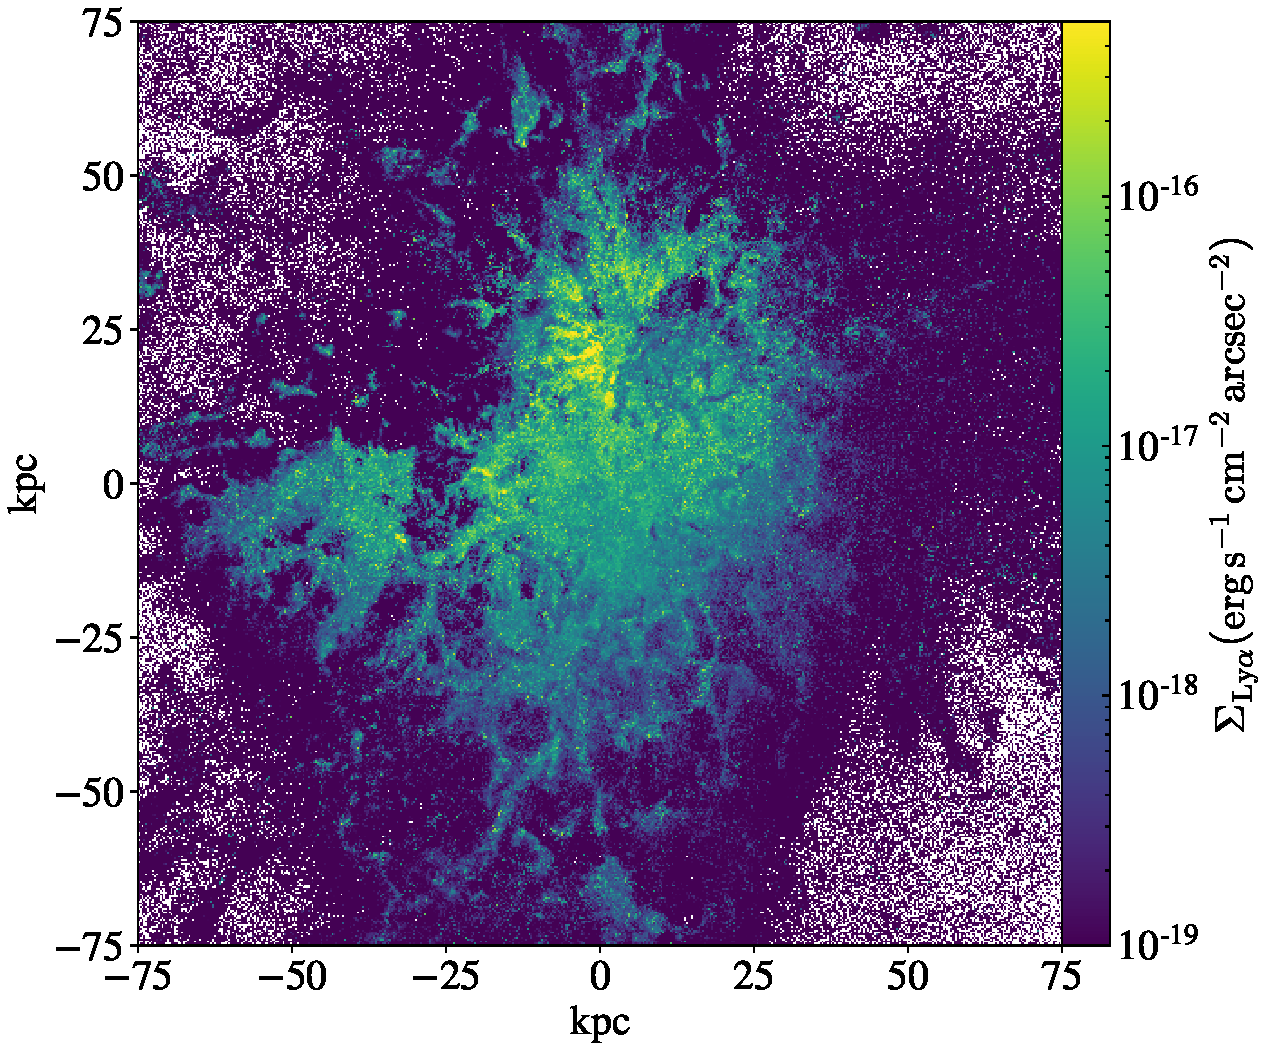
\includegraphics[width=\textwidth,height=\textheight,keepaspectratio]{figures/141.pdf}
    \caption{
        Example surface brightness image of a LAB where the luminosity is concentrated, which indicates the presence of an AGN, but the luminosity is not in a connected region.
    }
    \label{fig:agn_on_example}
\end{figure}

\begin{figure}
    \centering
    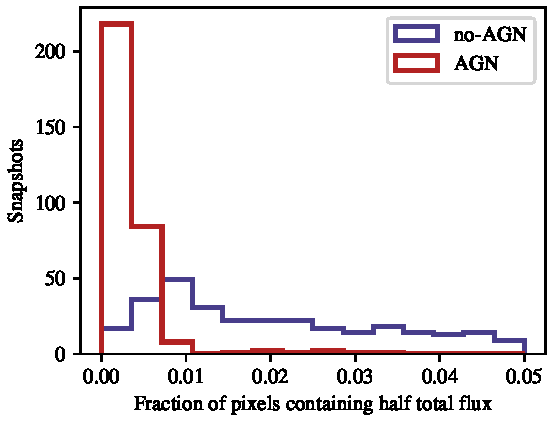
\includegraphics[width=\textwidth,height=\textheight,keepaspectratio]{figures/skew_distribution.pdf}
    \caption{
        We propose a metric for determining the presence of an AGN in an observed LAB: The fraction of all flux that is concentrated within a small fraction of the total area of the blob.
    In this figure since we are making a suggestion for an observable metric we have computed this metric on simulated surface brightness images after convolving to the resolution of MUSE.
    For the purpose of this demonstration we plot the fraction of pixels containing 50\% total flux but one could choose another threshold and find similar results.
    }
    \label{fig:skewness}
\end{figure}

\section{Impact of AGN model}
